\setcounter{section}{16}
\section{Попытка построить матрицу для $n = 2^k$ путем наложения единиц на минус единицы (получается только $k$ строчек). Решение для $n = 2^k$ через кронекеровское произведение.}
\par \textbf{"Наивный подход":} возьмем первую строчку состоящую только из 1, вторую - первая половина из единиц, вторая из минус единиц. Повторяем те же действия с каждой из полученных половин (делаем так чтобы каждая половина давала вклад ноль в скалярное произведение). Так как мы каждый раз увеличиваем количество блоков из одной и той же цифры в строке в $2$ раза, то через $k$ шагов мы получим строку в которой будут чередоваться $1$ и $-1$ и продолжить процесс мы не сможем.
\begin{figure}[h]
\center{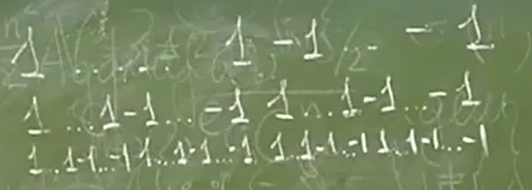
\includegraphics{images/17}}
\end{figure}

% \par $\blacktriangle$ Рассмотрим две произвольные строки $C$ с номерами $kb+l, pb+q$. Тогда их скалярное произведение равно
% $$a_{k1}a_{p1}(b_l, b_q) + a_{k2}a_{p2}(b_l, b_q) + \ldots + a_{ka}a_{pa}(b_l, b_q) = (b_l, b_q)(a_k, a_p)$$
% \par Так как мы берем 2 разные строчки, то либо $l \neq q$, либо $k \neq p$. Значит, так как $A, B$ - матрицы Адамара либо $(b_l, b_q)=0$, либо $(a_k, a_p)=0 \Rightarrow (c_{kb+l}, c_{pb+q})=0 \; \forall kb+l \neq pb+q \Rightarrow \quad C$ - матрица Адамара $\blacksquare$
\par \textbf{Конструктивный подход:} Воспользуемся определением кронекеровского произведения и утверждением о том, что кронекеровское произведение матриц Адамара является матрицей Адамара (см. билет 53):
$$H_4=H_2 \otimes H_2$$
$$\ldots$$
$$H_{2^k}=H_{2^{k-1}} \otimes H_2$$